%iffalse%\let\negmedspace\undefined
\let\negthickspace\undefined
\documentclass[journal,12pt,onecolumn]{IEEEtran}
\usepackage{cite}
\usepackage{amsmath,amssymb,amsfonts,amsthm}
\usepackage{algorithmic}
\usepackage{graphicx}
\usepackage{textcomp}
\usepackage{xcolor}
\usepackage{subcaption}
\usepackage{float}
\usepackage{caption}
\usepackage{txfonts}
\usepackage{listings}
\usepackage{titlesec}
\renewcommand{\thesubsection}{\thesection.\arabic{subsection}}
\titleformat{\subsection}
{\normalfont\bfseries\raggedright}
{\thesubsection}{1em}{}
\usepackage{enumitem}
\usepackage{mathtools}
\usepackage{gensymb}
\usepackage{comment}
\usepackage{ragged2e}
\usepackage{tfrupee}
\usepackage[breaklinks=true]{hyperref}
\usepackage{tkz-euclide} 
\usepackage{listings}
\usepackage{gvv}                                        
%\def\inputGnumericTable{}                                 
\usepackage[latin1]{inputenc}   
\usepackage{xparse}
\usepackage{color}                                            
\usepackage{array}                                            
\usepackage{longtable}                                       
\usepackage{calc}                                             
\usepackage{multirow}
\usepackage{multicol}
\usepackage{hhline}                                           
\usepackage{ifthen}                                           
\usepackage{lscape}
\usepackage{tabularx}
\usepackage{array}
\usepackage{float}
\newtheorem{theorem}{Theorem}[section]
\newtheorem{problem}{Problem}
\newtheorem{proposition}{Proposition}[section]
\newtheorem{lemma}{Lemma}[section]
\newtheorem{corollary}[theorem]{Corollary}
\newtheorem{example}{Example}[section]
\newtheorem{definition}[problem]{Definition}
\newcommand{\BEQA}{\begin{eqnarray}}
\newcommand{\EEQA}{\end{eqnarray}}
\usepackage{float}
%\newcommand{\define}{\stackrel{\triangle}{=}}
\theoremstyle{remark}
\usepackage{ circuitikz }
%\newtheorem{rem}{Remark}
% Marks the beginning of the document this one
\title{ EE1030 : SOFTWARE ASSIGNMENT}
\author{EE25BTECH11018 -- Darisy Sreetej}
\begin{document}
\maketitle

 \centering{\textbf{IMAGE COMPRESSION USING TRUNCATED SVD}}
\section{\textbf{Introduction}}
\vspace{1em}
\begin{justify}
    
Image compression aims to minimize storage requirements by expressing image data with fewer elements while maintaining visual quality. Through Singular Value Decomposition (SVD), an image matrix can be reconstructed using only its dominant singular values. This approach effectively preserves the main structure and details of the image in a compact form. The project applies truncated SVD to compress grayscale images and evaluates its accuracy for various rank values $k$

\end{justify}
\vspace{1em}
\section{\textbf{Summary of Strang's video}}
\vspace{1em}
 \begin{justify}
    The Singular Value Decomposition (SVD) is a fundamental way to break down any real matrix $\vec{A} \in \mathbb{R}^{m \times n}$ into simpler components as 
     \begin{align*}
         \vec{A} = \vec{U}\vec{S}\vec{V^T}
     \end{align*}
     where $\vec{U}$ , $\vec{V}$ are orthogonal matrices satisfying $\vec{U^T}\vec{U} = \vec{I_m} $   and $\vec{V^T}\vec{V} = \vec{I_n} $ The columns of $\vec{U}$ are called the left singular vectors, and they represent orthogonal directions in the output space, while the columns of $\vec{V}$ are the right singular vectors, representing orthogonal directions in the input space. The diagonal matrix 
  $\vec{S}$ contains singular values $\sigma_1 \ge \sigma_2 \ge \cdots \ge \sigma_r > 0$,which indicate the relative importance of each pair of singular vectors.
 \end{justify}
\vspace{1em}
\section{\textbf{Algorithms}}
\vspace{1em}
\begin{justify}
    Various algorithms exist to compute eigen values and eigen vectors. The following shows some widely used algorithms 

    \begin{enumerate}
        \item \textbf{QR Algorithm :} This algorithm iteratively decomposes $\vec{A}=\vec{QR}$ (where $\vec{Q}$ is orthogonal and $\vec{R}$ is upper triangular) and updates $\vec{A} \leftarrow \vec{R}\cdot \vec{Q}$ . The process converges to a triangular matrix , with eigen values on its diagnol.
        \item \textbf{Power iteration :} This iterative algorithm computes the dominant eigenvalue (largest by magnitude) and its corresponding eigenvector. Starting with an arbitrary vector $\vec{x}$ , the method repeatedly multiplies $\vec{A}\cdot \vec{x}$ and normalizes the result.
        \item \textbf{Jacobi method :} Designed for symmetric matrices, this algorithm zeroes out off-diagonal elements iteratively using Givens rotations. It converges to a diagonal matrix with eigenvalues on the diagonal.
        \item \textbf{Schur Decomposition :} The Schur decomposition decomposes a matrix $\vec{A}$ as $\vec{A} = \vec{Q}\vec{T}\vec{Q^*}$, where $\vec{Q}$ is a unitary matrix and $\vec{T}$ is a upper triangular matrix . The eigen values of  $\vec{A}$ are found on diagnols of $\vec{T}$
    \end{enumerate}
\end{justify}

\newpage

\section{\textbf{Why do I choose Power iteration ?}}
\vspace{1em}
\begin{justify}
    I selected Power Iteration method because because it offers a simple and intuitive way to estimate the largest singular values and their corresponding vectors without involving complicated matrix factorizations.It is computationally effecient for large , sparse matrices. The method relies on basic operations such as matrix vector multiplication and normalization, making it easy to implement and understand. Overall, it provides a good balance between accuracy and computational cost, which makes it an ideal choice for truncated SVD based image compression.
\end{justify}
\vspace{1em}
\section{\textbf{Power iteration}}
\vspace{1em}
\subsection{MATH}
\vspace{1em}
\begin{justify}

To find the Truncated SVD (Singular Value Decomposition) of an image matrix $\vec{A}$, which is represented by the approximation
\begin{align*}
         \vec{A} = \vec{U}\vec{S}\vec{V^T}
     \end{align*}
The singular values of $\vec{A}$ ($\sigma_i$) are the square roots of the eigenvalues ($\lambda_i$) of the matrix $\vec{B} = \vec{A^T}\vec{A}$.The right singular vectors of $\vec{A}$ ($v_i$) are the eigen vectors of matrix $\vec{B} $.Since $\vec{B}$ is a symmetric positive semi-definite matrix, the Power Iteration method can be efficiently used to find its dominant (largest) eigenvalue and eigenvector.\\
The standard Power Iteration algorithm iteratively approximates the dominant eigenvalue $\lambda_1$ and its corresponding eigenvector $\vec{v_1}$ of a symmetric matrix $\vec{B} \in \mathbb{R}^{n \times n}$.

\begin{enumerate}
    \item \textbf{Initialization:} Choose an arbitrary, non-zero starting vector $\vec{v^{(0)}}$.
    \item \textbf{Iteration:} The core iterative step is defined by:
    $$
    \vec{w^{(j+1)}} = \vec{B} \vec{v^{(j)}}
    $$
    $$
    \vec{v^{(j+1)}} = \frac{\vec{w^{(j+1)}}}{\norm{\vec{w^{(j+1)}}}}
    $$
    where $j$ is the iteration count, $\vec{v^{(j)}}$ is the current eigenvector estimate, and $\norm{\vec{w^{(j+1)}}}$ is the Euclidean (or $L_2$) norm used for normalization. The normalization step ensures numerical stability and prevents the vectors from growing indefinitely.
    \item \textbf{Eigenvalue Estimation:} As $j \to \infty$, $\vec{v^{(j)}}$ converges to the dominant eigenvector $\vec{v_1}$. The dominant eigenvalue $\lambda_1$ can be estimated using the Rayleigh quotient:
    $$
    \lambda_1 \approx \frac{(\vec{v^{(j)}})^T \vec{B} \vec{v^{(j)}}}{\norm{\vec{v^{(j)}}}} = (\vec{v^{(j)}})^T \vec{B} \vec{v^{(j)}}
    $$
    (Since $\vec{v^{(j)}}$ is a unit vector, $\norm{\vec{v^{(j)}}}$.
    \item\textbf{Deflation :}
    To find the subsequent eigenpairs $(\lambda_2, \vec{v_2})$, $(\lambda_3, \vec{v_3})$, and so on, we use \textbf{Deflation} technique. Once the $t$-th eigenpair $(\lambda_t, \vec{v_t})$ is found, we subtract its contribution from the original matrix $\vec{B}$ to create a new matrix $\vec{B^*}$ that has the same eigenvectors as $\vec{B}$, but where $\lambda_t$ is replaced by zero.

The deflated matrix $\vec{B_{t+1}}$ is computed from the previously used matrix $\vec{B_t}$ and the calculated eigenpair $(\lambda_t, \vec{v_t})$ as follows:
$$
\vec{B_{t+1}} = \vec{B_t} - \lambda_t \vec{v_t} \vec{v_t^T}
$$
where $\vec{B_1} = \vec{B}$. The Power Iteration is then applied to the deflated matrix $\vec{B_{t+1}}$ to find the next largest eigenpair, $(\lambda_{t+1}, \vec{v_{t+1}})$.
\item \textbf{SVD Calculation :}
After computing the $t$-th eigenpair $(\lambda_t, \vec{v_t})$ of $\vec{B}=\vec{A^T}\vec{ A}$:

     The $t$-th singular value is $\sigma_t = \sqrt{\lambda_t}$.
     The $t$-th right singular vector is $\vec{v_t}$ (the normalized eigenvector).
     The $t$-th left singular vector $\vec{u_t}$ is computed using the SVD definition $\vec{A} \vec{v_t} = \sigma_t \vec{u_t}$:
    $$
    \vec{u_t} = \frac{\vec{A} \vec{v_t}}{\sigma_t}
    $$
    This vector $\vec{u_t}$ must also be normalized to ensure it is a unit vector.
   \end{enumerate}
   \end{justify}
   \vspace{1em}
\subsection{PSEUDO-CODE}
\vspace{1em}
\begin{justify}
    \begin{enumerate}
        \item \textbf{Function 1: (normalization)}\\
        \vspace{0.5em}
        Input: vector v of length n \\
      Output: normalized vector v (unit length)

     Procedure:\\
    1. Compute magnitude = sqrt( sum of $\vec{v[i]^2}$ for all $i$ ) \\
    2. If magnitude $>$ EPS:\\
      For each element $i$ :
          $\vec{v[i]}$ = $\vec{v[i]}$ / magnitude
\vspace{0.5em}
 \item \textbf{Function 2: (matrix-vec)}\\
 \vspace{0.5em}
Input: matrix $\vec{M}$ of size $m*n$, vector $\vec{v}$ of length n \\
Output: result = $\vec{M} \cdot \vec{v} $(length m)

Procedure:\\
For each row i from 0 to $m-1$:\\
$\vec{result[i]}$ = 0\\
For each column j from 0 to $n-1$:\\
$\vec{result[i]} += \vec{M[i*n + j]} * \vec{v[j]}$

 \vspace{0.5em}
\item \textbf{Function 3 : (pow-iter)}\\
 \vspace{0.5em}
Input: square matrix $\vec{N}$ $(n*n)$\\
Output: dominant eigenvalue $\lambda$ and eigenvector $\vec{v}$\\

Procedure:\\
1. Initialize $\vec{v}$ randomly and normalize($\vec{v}$)\\
2. Repeat for MAX iterations:\\
      $\vec{x} = \vec{N} \cdot \vec{v} $ \\
      normalize($\vec{x}$)\\
      $\vec{v} = \vec{x}$\\
3. Compute $\vec{x} = \vec{N}\cdot \vec{v}$\\
4. eigen-val = $\vec{v^T}\cdot\vec{x}$   (Rayleigh quotient)\\
5. Return eigen-val  (largest eigenvalue)

\item \textbf{Funtion 4 : (svd-reconstructed)}\\
Input:\\
  $\vec{A}$ : matrix of size ($\vec{r} \cdot \vec{c}$)\\
  $k$ : number of singular components to retain\\

Output:\\
  A-recon : rank-k reconstructed approximation of A\\
Procedure:\\
1. Allocate matrices:\\
      $\vec{B}$  = $c*c$ matrix\\
      $\vec{B1}$ = working copy of $B$\\
      $\vec{U}$  = $r*k$\\
      $\vec{V}$  = $c*k$\\
      $\vec{S}$  = k-element vector\\
      $\vec{v}$  = c-element vector\\
      $\vec{u}$  = r-element vector\\
2. Compute $\vec{B} = \vec{A^T} \vec{A}$\\
      For each $i,j$:\\
          $B_(ij)$ = sum over $\vec{p}$ of ( $\vec{A_(pi)} * \vec{A_(pj)} $)\\
3. Copy $\vec{B}$ into $\vec{B1}$  ($\vec{B1}$ will be deflated during iteration)\\
4. For each component $t = 0$ to $k-1$:\\
      a) eigen-val = pow-iter($\vec{B1}$, c, $\vec{v}$)\\
      b) S[t] = sqrt(eigen-val)\\
      c) Store $\vec{v}$ as column t of $\vec{V}$\\
      d) Deflate $\vec{B1}$ = $\vec{B1} - eigen-val\cdot\vec{v}\cdot\vec{v^T}$\\
         (Removes the influence of this eigenvector)\\
5. Compute $\vec{U}$ (left singular vectors)\\
      For each t = 0 to $k-1$:\\
          $\vec{v}$ = column t of $\vec{V}$\\
          $\vec{u} = \vec{A}\cdot \vec{v}$\\
          normalize($\vec{u}$)\\
          Store $\vec{u}$ as column t of $\vec{U}$\\
6. Reconstruct A-recon = $\vec{U}\vec{S}\vec{V^T}$\\
      For each pixel position (b, d):\\
          A-recon[b, d] = sum over $i= 0 \rightarrow k-1$ of\\
                           $\vec{U[bi]} \vec{S[i]} \vec{V[di]}$ \\
7. Free all allocated memory\\
\item \textbf{Python :}
\begin{enumerate}
\item  Load grayscale image and convert to float64 matrix $\vec{A}$.
\item  Make $\vec{A}$ C-contiguous for ctypes.
\item  Create an empty matrix $\vec{A_r}$ of same size.
\item  Load shared library svd-compression.so.
\item  Define C function argument types and restype = None.
\item  Set k = min(k, rows, cols).
\item Call svd-reconstructed(A, rows, cols, k, $\vec{A_r}$).
\item  Compute Frobenius error = sqrt(sum($({A} - {A_r})^2$)).
\item  Print k and error value.
\item  Compare original and reconstructed images

\end{enumerate}
    \end{enumerate}
\end{justify}

\newpage

\section{\textbf{Implementation}}
\begin{justify}

Let us take an example image for implementation  \\
If we take an image "einstein.jpg" and set k=20 , we get the following results through the code \\

\begin{figure}[H]
    \centering
    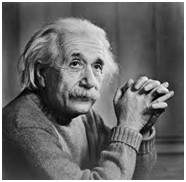
\includegraphics[width=0.37\linewidth]{figs/original/einstein.jpg}
    \caption{Original}
    \label{fig:placeholder}
\end{figure}

\begin{figure}[H]
\centering
\begin{subfigure}{0.22\textwidth}
    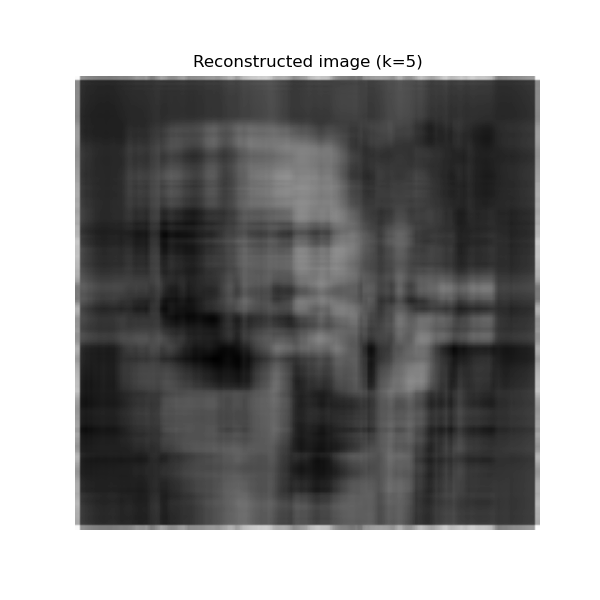
\includegraphics[width=\linewidth]{figs/reconstructed/einstein_k5.png}
    \caption{k=5}
\end{subfigure}
\hfill
  \begin{subfigure}{0.22\textwidth}
    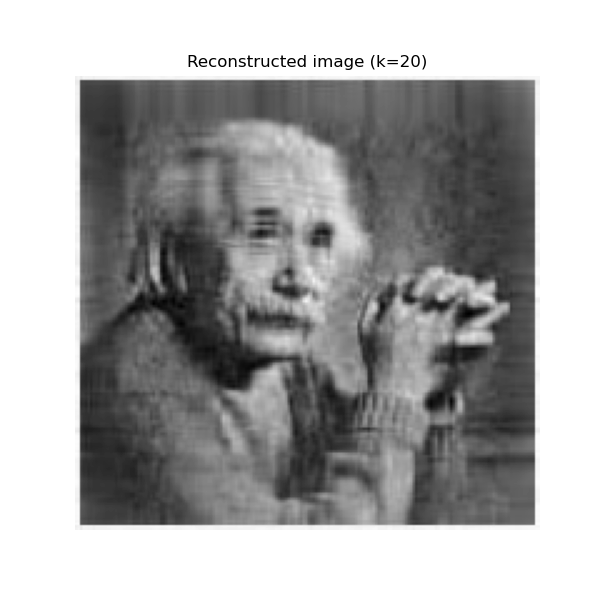
\includegraphics[width=\linewidth]{figs/reconstructed/einstein_k20.png}
    \caption{k=20}
\end{subfigure}
\hfill 
  \begin{subfigure}{0.22\textwidth}
    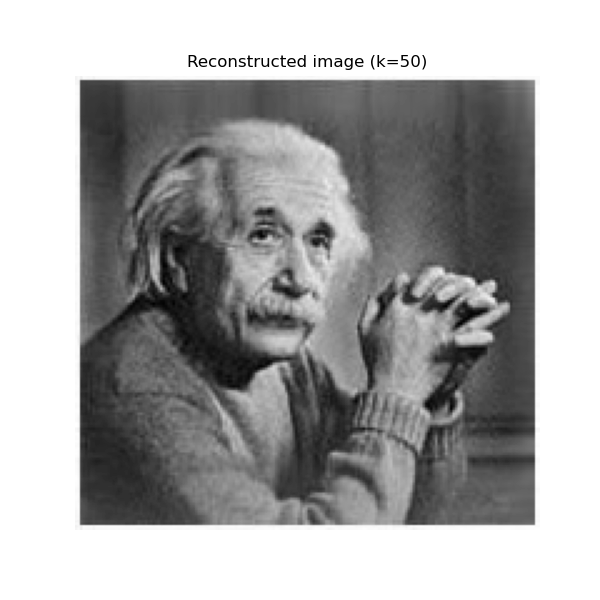
\includegraphics[width=\linewidth]{figs/reconstructed/einstein_k50.png}
    \caption{k=50}
\end{subfigure}
\hfill 
  \begin{subfigure}{0.22\textwidth}
    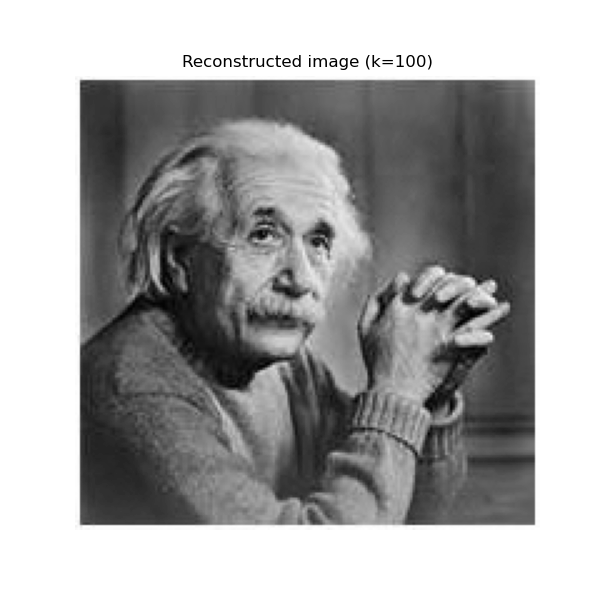
\includegraphics[width=\linewidth]{figs/reconstructed/einstein_k100.png}
    \caption{k=100}
\end{subfigure}
\hfill 
\end{figure}


Similarly , we will get the results for remaining images with assigned k value of our choice .
\end{justify}

\section{\textbf{Error Analysis}}

\begin{justify}
The \textbf{Frobenius error} (or Frobenius norm of the difference) measures how close the reconstructed matrix $\vec{A_k}$ is to the original matrix $\vec{A}$ 

\begin{align*}
    \norm{\vec{E}}_F = \norm{\vec{A} - \vec{A_k}}_F
\end{align*}
It keeps on changing for different images . As $k$ increases $\rightarrow$ reconstruction improves $\rightarrow$ Frobenius error decreases.\\
\vspace{0.5em}

\begin{table}[H]
\begin{minipage}[t]{0.32\textwidth}
    \centering
    \begin{tabular}[12pt]{ |c| c| }
    \hline
    {$k$} & {Frobenius error}\\ 
    \hline
    5 & 4713.338823 \\
    \hline
    20 & 2126.439196 \\
    \hline
    50 & 880.355637 \\
    \hline
    100 & 164.818244 \\
    \hline
\end{tabular}

    \caption*{einstein.jpg}
\end{minipage} 
\hfill
\begin{minipage}[t]{0.3\textwidth}
    \centering
   \begin{tabular}[12pt]{ |c| c| }
    \hline
    {$k$} & {Frobenius error}\\ 
    \hline
    5 &   20703.892759\\
    \hline
    20 &  10633.922961 \\
    \hline
    50 &  6185.247394 \\
    \hline
    100 & 3672.739859 \\
    \hline
\end{tabular}

    \caption*{globe.jpg}
\end{minipage}
\hfill
\begin{minipage}[t]{0.3\textwidth}
    \centering
  \begin{tabular}[12pt]{ |c| c| }
    \hline
    {$k$} & {Frobenius error}\\ 
    \hline
    5 &  11151.980266 \\
    \hline
    20 &  3808.753741 \\
    \hline
    50 &  1158.834821 \\
    \hline
    100 & 511.562193 \\
    \hline
\end{tabular}

   \caption*{greyscale.png}
\end{minipage}

\caption{Frobenius error for different images}

\end{table}

\end{justify}
\section{\textbf{Conclusion}}
\begin{justify}
\begin{enumerate}
    \item 
    This project successfully implemented a low-rank approximation of a grayscale image matrix using the \textbf{Truncated Singular Value Decomposition} (SVD), with the top $k$ singular values and vectors computed entirely in C using the \textbf{Power Iteration} method with  Deflation.

\item The choice of Power Iteration was justified by its straight forward implementation and relative ease of parallelization, though it necessitates working with the $\vec{A^T A}$ matrix, which can square the condition number and thus increase numerical error compared to direct SVD methods.
\item Despite this theoretical limitation, the hybrid C/Python implementation demonstrated effective and numerically stable extraction of the dominant eigenpairs required for compression.

\item The results, documented in the preceding sections, clearly illustrate the fundamental trade-off of image compression using SVD: as the rank $k$ increases, the Frobenius norm error $||A-A_k||_{F}$ rapidly decreases, leading to higher image fidelity. 


\end{enumerate}
\end{justify}


\end{document}